\documentclass[11pt]{article}

% Layout and typography
\usepackage[a4paper,left=2cm,right=2cm,top=2.5cm,bottom=2.5cm]{geometry}
\linespread{1.25}
\setlength{\parindent}{0pt}
\setlength{\parskip}{6pt plus 2pt minus 1pt}

% Figures and tables
\usepackage{graphicx}
\usepackage{float}
\usepackage{rotating}
\usepackage{booktabs}
\usepackage{multirow}
\usepackage{longtable}
\usepackage{array}
\usepackage{placeins}
\usepackage{caption}
\usepackage{subcaption}
\usepackage{tikz}

% References / language
\usepackage[natbibapa]{apacite}
\usepackage[english]{babel}
\usepackage[autostyle, english=american]{csquotes}

% Math and colors
\usepackage{amsmath}
\usepackage{xcolor}

% Colours we use
\definecolor{occblue}{HTML}{273A8F}
\definecolor{occgreen}{HTML}{2C5C34}
\definecolor{occred}{HTML}{B33D3D}
\definecolor{occorange}{HTML}{DE7500}

\newcommand{\co}[1]{{\color{red}\textbf{[}#1\textbf{]}}}

\interfootnotelinepenalty=10000
\widowpenalties 1 10000

\begin{document}

\begin{center}
    \LARGE
    \textbf{Solution Note} \\

    \vspace{0.5cm}

    \large
    \textbf{Solution to the practice problem related to the addition rule on slide 38 in ``02 Uncertainty and probability''} \\

    \vspace{0.5cm}

    2026-02-13

    \vspace{0.5cm}

    \large
    Christian Vedel,\\
    \vspace{0.125cm}
    Department of Economics \\
    University of Southern Denmark
\end{center}

\vspace{0.5cm}

In the lecture we discussed a problem that caused some confusion. During class it was suggested that the problem contained an error. That was not accurate. There is no error in the problem. However, it \emph{is} a bit confusing.

The problem is about accounting for probabilities related to students and their line of study. The confusion arises because it is easy to overlook that some students may be in neither category.

This is a valuable exercise because it presents an apparent paradox. The paradox is resolved because the tools introduced so far allow us to recover \textit{hidden information about the students studying neither}.

The note is structured as follows. Section 1 outlines the problem. Section 2 outlines the solution. Section 3 explains the apparent paradox and resolves it.

\section{Problem}
The problem given in the lecture is the following:

\begin{center}
\fbox{
\parbox{0.70\textwidth}{
\textit{In a class of 30 students:}
\begin{itemize}
    \item 18 students study economics
    \item 12 students study statistics
    \item 8 students study both economics and statistics
\end{itemize}

Let $A$ = ``studies economics'' and $B$ = ``studies statistics''

\begin{enumerate}
    \item What is $P(A)$, $P(B)$, and $P(A \cap B)$?
    \item Use the addition rule to find $P(A \cup B)$ — the probability that a randomly selected student studies economics or statistics (or both).
    \item What is $P(A^c)$? Interpret this in words.
\end{enumerate}
}
}
\end{center}

\section{Solution}

\subsection{Q1}
Since $A$ = ``studies economics'' and $B$ = ``studies statistics'', we have
\begin{equation}
\begin{split}
    P(A)&=\frac{18}{30}, \\
    P(B)&=\frac{12}{30}.
\end{split}
\label{eq:e1}
\end{equation}

The event $A \cap B$ consists of those students who study both. This is given directly in the problem statement:
\begin{equation}
\begin{split}
    P(A \cap B)&=\frac{8}{30}.
\end{split}
\label{eq:e2}
\end{equation}

\subsection{Q2}
This question asks for the probability that a student studies economics or statistics, i.e.\ the event $A \cup B$. In other words: what share of students study economics, statistics, or both?

\textcolor{occred}{It is easy to think that the answer should be \textit{all of them} — $\frac{30}{30}$. But that turns out not to be the case. More about this in Section~3.}

From the addition rule,
\begin{equation}
\begin{split}
    P(A\cup B)=P(A)+P(B)-P(A \cap B).
\end{split}
\label{eq:e3}
\end{equation}

Using the results from Q1,
\begin{equation}
\begin{split}
    P(A\cup B)&=P(A)+P(B)-P(A \cap B) \\
    &=\frac{18}{30} + \frac{12}{30} - \frac{8}{30} \\
    &=\frac{30}{30} - \frac{8}{30} \\
    &=\frac{22}{30} \approx 0.7333.
\end{split}
\label{eq:e4}
\end{equation}

The intuition behind Equation~\ref{eq:e3} is the following. We want to count everyone in $A$ and everyone in $B$. But students in $A \cap B$ would be counted twice:

\textit{When we count the students in $A$}, we also include those in $A\cap B$. In words: some economics students are also statistics students.

\textit{When we count the students in $B$}, we also include those in $A\cap B$. In words: some statistics students are also economics students.

Therefore, adding $P(A)$ and $P(B)$ double-counts the overlap. To correct for this, we subtract $P(A\cap B)$ once.

\subsection{Q3}
In this question we are asked to find the share of students in the complement of $A$, denoted $A^c$. That is, the students who \emph{do not} study economics.

A general rule (see slide 37) is:
\begin{equation}
\begin{split}
    P(A^c)=1 - P(A).
\end{split}
\label{eq:e5}
\end{equation}

Using the result from Q1,
\begin{equation}
\begin{split}
    P(A^c)&=1 - \frac{18}{30} \\
    &=\frac{12}{30} = 0.4.
\end{split}
\label{eq:e6}
\end{equation}

Interpretation: $P(A^c)=0.4$ means that 40\% of the class does \emph{not} study economics. In this setting, that includes students who study statistics only \emph{and} students who study neither economics nor statistics.

\section{The paradox}
Below are three different explanations of the same point. Each one of them offers a different lense for seing the paradox and why it is resolved. 

\subsection{Explanation 1: Account for all students (the $2\times 2$ table)}
At first glance, the numbers can feel contradictory. There are 18 economics students and 12 statistics students, so it is tempting to think that \emph{everyone} must be in at least one of the two groups.

The key is that the 8 students who study both are included in \emph{both} counts. This is why the addition rule subtracts the overlap once:
\[
18 + 12 - 8 = 22.
\]
So only 22 of the 30 students are in $A \cup B$. The remaining
\[
30 - 22 = 8
\]
students are in neither category.

It can help to lay out all groups explicitly:
\begin{itemize}
    \item Economics only: $18-8=10$
    \item Statistics only: $12-8=4$
    \item Both: $8$
    \item Neither: $30-(10+4+8)=8$
\end{itemize}

These numbers are consistent with the original information, and they show where the ``missing'' students are:

\begin{center}
\begin{tabular}{lccc}
\toprule
 & Statistics: yes & Statistics: no & Total \\
\midrule
Economics: yes & 8 & 10 & 18 \\
Economics: no  & 4 & \textbf{\textcolor{occred}{8}}  & 12 \\
\midrule
Total          & 12 & 18 & 30 \\
\bottomrule
\end{tabular}
\end{center}

The apparent paradox disappears once we recognize that the problem statement does not say that every student studies economics or statistics. The addition rule reveals (and quantifies) the students who study neither.

\subsection{Explanation 2: Why subtraction is needed (double-counting)}
Imagine listing the economics students on one sheet of paper (18 names) and the statistics students on another sheet (12 names). If you stack the two sheets and count names, any student who is on \emph{both} sheets will be counted twice.

The overlap is 8 names, so $18+12$ counts 8 students twice. Subtracting 8 removes the extra copies:
\[
|A\cup B| = 18+12-8 = 22.
\]
So the class has 22 students in at least one of the two groups, and the remaining $30-22=8$ students are in neither group.

\subsection{Explanation 3: Venn diagram}
A Venn diagram makes the bookkeeping visual. The overlap (8 students) belongs to both sets, so it gets counted twice if we simply add 18 and 12. The addition rule subtracts the overlap once to correct this.

\begin{center}
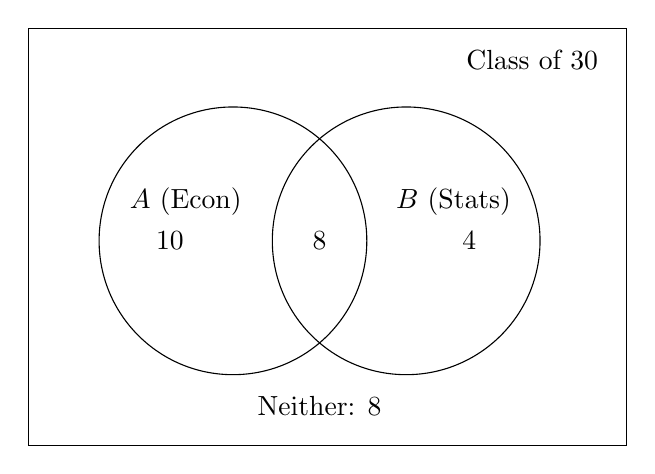
\begin{tikzpicture}[scale=1]
  % Universe
  \draw (-2.6,-2.6) rectangle (5,2.7);
  \node at (3.8,2.3) {Class of 30};

  % Circles
  \draw (0,0) circle (1.7);
  \draw (2.2,0) circle (1.7);

  % Labels for sets
  \node at (-0.6,0.5) {$A$ (Econ)};
  \node at (2.8,0.5) {$B$ (Stats)};

  % Region counts
  \node at (-0.8,0) {10};
  \node at (1.1,0) {8};
  \node at (3.0,0) {4};

  % Outside count
  \node at (1.1,-2.1) {Neither: 8};
\end{tikzpicture}
\end{center}

From the diagram,
\[
|A\cup B| = 10 + 8 + 4 = 22,
\qquad
30-22 = 8 \text{ study neither.}
\]

\end{document}
